% % % % % % % % % % % % % % % % % % % % % % % % % % % % % % % % % % % % % % % % 
% Formelsammlung von LaTeX4EI									
%
% @encode: 	UTF-8, tabwidth = 4, newline = LF
% @author:	Emanuel Regnath
% @date:		
%
% % % % % % % % % % % % % % % % % % % % % % % % % % % % % % % % % % % % % % % % 

%---------------------------------------%
%				Werkstoffe				%
%~~~~~~~~~~~~~~~~~~~~~~~~~~~~~~~~~~~~~~~%

% Document Class ===============================================================
\documentclass[fs, footer]{latex4ei}

% DOCUMENT_BEGIN ===============================================================
\begin{document}

% Split in 4 Columns ===========================================================
\begin{multicols*}{4}

% TITLE ========================================================================
\fstitle{Werkstoffe}


% Login: studentei
% PWd: WdE-2011#

%====================================
% Konstanten und Basisgleichungen |
%====================================
% Alle häufig gebrauchten Konstanten und Basisgleichungen

\section{Mathematische Grundlagen}
\sectionbox{
\subsection{Sinus, Cosinus \quad $\sin^2(x) \bs + \cos^2(x) = 1$}
%\begin{center}
%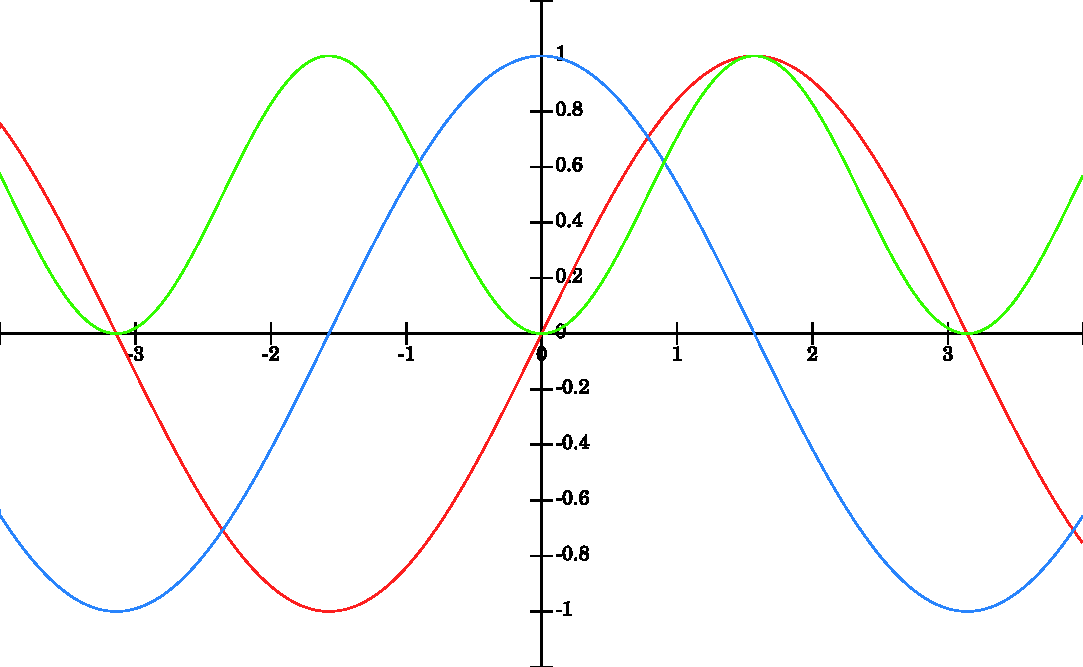
\includegraphics[width=4.4cm]{./img/sinus.pdf}
%\end{center}

\setlength{\tabcolsep}{4pt}
\tablebox{
\begin{tabular*}{\columnwidth}{@{\extracolsep\fill}c|c|c|c|c||c|c|c|c@{}} \ctrule
$x$ & $0$ & $\pi / 6$ & $\pi / 4$ & $\pi / 3$ & $\frac{1}{2}\pi$ & $\pi$ & $1\frac{1}{2}\pi$ & $2 \pi$ \\
$\scriptstyle{ \varphi }$ & $\scriptstyle{0^\circ}$ & $\scriptstyle{30^\circ}$ & $\scriptstyle{45^\circ}$ & $\scriptstyle{60^\circ}$ & $\scriptstyle{90^\circ}$ & $\scriptstyle{180^\circ}$ & $\scriptstyle{270^\circ}$ & $\scriptstyle{360^\circ}$ \\ \cmrule
$\sin$ & $0$ & $\frac{1}{2}$ & $\frac{1}{\sqrt{2}}$ & $\frac{\sqrt 3}{2}$ & $1$ & $0$ & $-1$ & $0$ \\
$\cos$ & $1$ & $\frac{\sqrt 3}{2}$ & $\frac{1}{\sqrt 2}$ & $\frac{1}{2}$ & $0$ & $-1$ & $0$ & $1$ \\     
$\tan$ & $0$ & $\frac{\sqrt{3}}{3}$ &	$1$	&	$\sqrt{3}$ & $\pm \infty$ & $0$ & $\mp \infty$ & $0$\\ \cbrule
\end{tabular*} }\\
\begin{tabular*}{\columnwidth}{@{\extracolsep\fill}ll@{}}
	Additionstheoreme &  Stammfunktionen\\
 	$\cos (x - \frac{\pi}{2}) = \sin x$ & $\int x \cos(x) \diff x = \cos(x) + x \sin(x)$\\
 	$\sin (x + \frac{\pi}{2}) = \cos x$ & $\int x \sin(x) \diff x = \sin(x) - x \cos(x)$\\
 	$\sin 2x = 2 \sin x \cos x $  & $\int \sin^2(x) \diff x = \frac12 \bigl(x - \sin(x)\cos(x) \bigr)$\\ 
 	$\cos 2x = 2\cos^2 x - 1$  & $\int \cos^2(x) \diff x = \frac12 \bigl(x + \sin(x)\cos(x) \bigr)$\\
 	$\sin(x) = \tan(x)\cos(x)$ & $\int \cos(x)\sin(x) = -\frac12 \cos^2(x)$ \\
 	\multicolumn{2}{l}{$\sin ( x \pm y ) = \sin x \; \cos y \pm \sin y \; \cos x$}\\
 	\multicolumn{2}{l}{$\cos ( x \pm y ) = \cos x \; \cos y \mp \sin x \; \sin y$}\\
\end{tabular*}
}

\sectionbox{
	\subsection{Integrale $\int e^x\;\mathrm{d} x = e^x = (e^x)'$}
	\tablebox{
	\renewcommand{\arraystretch}{1.6} 
	\begin{tabular*}{\columnwidth}{@{\hspace{5mm}}c@{\extracolsep\fill}c@{\extracolsep\fill}c@{\hspace{5mm}}} \ctrule
		$F(x)$ & $f(x)$ & $f'(x)$ \\ \cmrule
		$\frac{1}{q+1}x^{q+1}$ & $x^q$ & $qx^{q-1}$ \\
		\raisebox{-0.2em}{$\frac{2\sqrt{ax^3}}{3}$} & $\sqrt{ax}$ & \raisebox{0.2em}{$\frac{a}{2\sqrt{ax}}$}\\
		$x\ln(ax) -x$ & $\ln(ax)$ & $\textstyle \frac{a}{x}$\\
		%e^x & e^x & e^x \\
		$\frac{1}{a^2} e^{ax}(ax- 1)$ & $x \cdot e^{ax}$ & $e^{ax}(ax+1)$ \\
		$\frac{a^x}{\ln(a)}$ & $a^x$ & $a^x \ln(a)$ \\
		$-\cos(x)$ & $\sin(x)$ & $\cos(x)$\\ \cbrule
	\end{tabular*} }\\
	
	$\int e^{at} \sin(bt) \diff t = e^{at} \frac{a \sin(bt) + b \cos(bt)}{a^2 + b^2}$\\
	\begin{tabular*}{\columnwidth}{@{\extracolsep\fill}ll@{}}
	$\int \frac{\diff t}{\sqrt{at+b}} = \frac{2 \sqrt{at+b}}{a}$ & $\int t^2 e^{at} \diff t = \frac{(ax-1)^2+1}{a^3} e^{at}$\\
	$\int t e^{at} \diff t = \frac{at-1}{a^2} e^{at}$ & $\int x e^{ax^2} \diff x = \frac{1}{2a} e^{ax^2}$\\
	\end{tabular*}
}
	
\sectionbox{
\subsection{Exponentialfunktion und Logarithmus}
\begin{tabular*}{\columnwidth}{l@{\extracolsep\fill}ll}
	$a^x = e^{x \ln a}$ & $\log_a x = \frac{\ln x}{\ln a}$ & $\ln x \le x -1$\\
	$\ln(x^{a}) = a \ln(x)$ & $\ln(\frac{x}{a}) = \ln x - \ln a$ & $\log(1) = 0$\\
\end{tabular*}
}
\section{Einheiten}
%\sectionbox{
%\subsection{SI-Einheiten}
%\symbolbox{

%}
%}
\sectionbox{
\topicbox{SI-Präfixe}{
	\begin{tabular}{ccl|ccl}
	Symbol & Vorsatz & Faktor & Symbol & Vorsatz & Faktor \\
	Y&Yotta&$10^{24}$& d &Dezi&$10^{-1}$\\
	Z&Zetta&$10^{21}$& c &Zenti&$10^{-2}$\\
	E&Exa&$10^{18}$& m & Milli&$10^{-3}$\\
	P&Peta&$10^{15}$& $\mu$ & Mikro&$10^{-6}$\\
	T&Tera&$10^{12}$& n &Nano&$10^{-9}$\\
 	G&Giga&$10^9$& p &Piko&$10^{-12}$\\
	M&Mega&$10^6$& f &Femto&$10^{-15}$\\
	k&Kilo&$10^3$& a &Atto&$10^{-18}$\\
	h&Hekto&$10^2$& z & Zepto&$10^{-21}$\\
	da&Deka&$10^1$ & y &Yokto&$10^{-24}$\\
	\end{tabular}
}
}

\section{Konstanten und Basisgleichungen}
\sectionbox{
\topicbox{Naturkonstanten}{
	\begin{tabular}{rl}
		Lichtgeschwindigkeit & $\mathrm{c}_0 = \SI{299 792 458}{\meter\per\second}$\\
		Elementarladung & $\mathrm{e}  = \SI{1.602 177e-19}{\coulomb}$\\
		\textsc{Planck}-Konst. & $h = \SI{6,626 069 57e-34}{\joule\second}$\\
								& $\hbar = \frac{h}{2 \pi} = \SI{1.05457e-34}{\joule\second}$ \\
		Elektr. Feldkonst. & $\varepsilon_0 = \SI{8.854 188e-12}{\farad\per\meter}$\\
		Magn. Feldkonst. & $\mu_0 = 4\pi \times \SI{e-7}{\henry\per\meter}$\\
		\textsc{Avogadro}-Konst. & $N_A = \SI{6.022 141e23}{\per\mole}$\\
		Atomare Masse & $\mathrm{u} = \SI{1.660 539e-27}{\kilogram}$\\
		Elektronenmasse & $m_e = \SI{9,109 383e-31}{\kilogram}$\\
		Protonenmasse & $m_p = \SI{1,674 927e-27}{\kilogram}$\\
		Neutronenmasse & $m_n = \SI{1,672 622e-27}{\kilogram}$\\
		%Feinstruktur & $\alpha^{-1} = \num{137,035 999}$\\
		\textsc{Boltzmann}-Konst. & $k_b = \SI{1.380 655e-23}{\joule\per\kelvin}$\\
		allg. Gaskonstante & $R = k_b N_A= 8,3144 \frac{\text{J}}{\text{mol} \text{ K}}$ \\
	\end{tabular}
	}
}
% SECTION ====================================================================================
\section{Aufbau der Materie}
%=============================================================================================
\sectionbox{
\paragraph{Planck'sches Postulat} In der Quantenmechanik kann der harmonische Oszillator mit der Schwingungsfrequenz f nur diskrete Energiewerte annehmen:\\
$E_n = hf\left(n + \frac{1}{2}\right) = \hbar \omega \left(n + \frac{1}{2}\right)$
\paragraph{Heisenberg'sche Unschärferelation} Ort und Impuls (bzw. Energie und Zeit) können nicht gleichzeitig scharf definiert werden.\\
$\Delta x \cdot \Delta p \geq \frac{\hbar}{2}$ und $\Delta t \cdot \Delta E \geq \frac{\hbar}{2}$
\paragraph{Welle-Teilchen-Dualismus} Materie kann sowohl Eigenschaften von Teilchen als auch von Wellen haben.
}
\sectionbox{
\subsection{Quanten}
Hierbei wird die Materie als Menge von Teilchen betrachtet.\\
Sie haben eine Energie E und einen Impuls p sowie eine Masse m.
\paragraph{Das Photon} Für das Photon gilt:\\
$E_{\ir ph}=f\cdot h= \hbar \cdot \omega = \frac{hc}{\lambda} = m_{\text{ph}}c^2$ \\
$m_{\text{ph}} = \frac{\hbar \omega}{c^2}$  \qquad\qquad $p_{\text{ph}} = m_{\text{ph}} \cdot c = \frac{h}{\lambda}$
}

\sectionbox{
	\subsection{Materiewellen}
\subsubsection{Allgemeine Wellenfunktion $\Psi(\vec{r},t) = C \cdot e^{\i(\omega t - \vec{k} \cdot \vec{r})}$}
Im eindimensionalen Fall: 
$\Psi(x,t) = C \cdot e^{\i(\omega t - kx)}$

\tablebox{
		\begin{tabular*}{\columnwidth}{@{\extracolsep\fill}ll@{}}
		\ctrule
	Größe & Beziehung \\ \cmrule
	Energie & $E = \frac{1}{2}mv^2 = \hbar \omega$ \\
	De-Broglie-Wellenlänge & $\lambda = \frac{h}{p}$ \\
	Impuls & $\vec{p} = m \vec{v} = \hbar \vec{k}$ \\
	Kreisfrequenz & $\omega = 2 \pi f = \frac{\hbar}{2m} k^2$ \\
	Phasengeschwindigkeit & $v_{\text{ph}} = \frac{\omega}{k} = \frac{\hbar k}{2m} = \frac{v_{\text{Teilchen}}}{2}$ \\
	Wellenzahl & $k = \frac{2 \pi}{\lambda}$ \\
		\ctrule
		\end{tabular*}
	}
\subsubsection{Das Wellenpaket}
Der bewegten Korpuskel wird eine im Raum begrenzte Wellenfunktion zugeordnet, die sich aus der Überlagerung einzelner Wellen zu einem Wellenpaket ergibt. Ein Teilchenstrom entspricht der Folge einzelner Wellenpakete.

% Teilchenstrom entspricht Folge einzelner Wellenpakete.
$\Psi(\vec{r},t) = \int\limits_{k_0 - \Delta k}^{k_0 + \Delta k}{C(k) \cdot e^{\i (\omega t - \vec{k} \vec{r})} \diff k}$

Gruppengeschwindigkeit des Wellenpakets:

$v_{\text{gr}} = \frac{\diff \omega}{\diff k} = \frac{\hbar k}{m} = \frac{p}{m} = v_{\ir Teilchen}$

Phasengeschwindigkeit $v_{\text{ph}} = \frac{\omega}{k}$
} 


\sectionbox{
	\subsection{Die Schrödingergleichung}
Beschreibt die Dynamik der quantenmech. Zustände eines Systems.
\subsubsection*{Allgemeine Schrödingergleichung:}
$E = E_{\ir kin} + V_{\ir pot} = \frac{p^2}{2m} + V$ \qquad mit $p = \i \hbar \nabla \Psi$
\begin{center}
	\boxed{-\i \hbar \frac{\partial}{\partial t} \Psi ( \vec r , t ) = - \frac{\hbar^2}{2m} \lpo \Psi (\vec r, t) + V(\vec{r},t) \cdot \Psi (\vec r, t)}
\end{center} 

\subsubsection*{Zeitunabhängige Schrödingergleichung:} 
\begin{center}
	\boxed{- \frac{\hbar^2}{2m} \Delta \Psi (\vec r) = (E-V) \Psi(\vec r)}
\end{center} 

\paragraph{Herleitung} 	Durch den Separationsansatz $\Psi(\vec{r},t) = \Psi(\vec{r})\Phi(t)$ lässt sich die Zeitabhängigkeit abtrennen.
\paragraph{Aufenthaltswahrscheinlichkeit} $\diff w(\vec{r}) = \Psi^*(\vec{r},t) \cdot \Psi(\vec{r},t) \cdot \diff \tau$
% Falls E > V: \Psi = e^{\i k \omega t} (Oszillierende E-Funktion) 
% Falls E < V: \Psi = e^{\alpha + \i \beta} (Abklingende E-Funktion) 
% Klausur: Unendlicher Potentialtopf $E = $
\paragraph{Normierungsbedingung:} 
$\int\limits_{\text{Volumen}}^{}{\Psi^* \Psi \diff r'} = 1$ \qquad $\Ra C_i = \sqrt{\frac{2}{L_i}}$
 \\ 

	\cookbox{Herleitung der Schrödingergleichung}{
	\item Aus De-Broglie-Beziehungen: 
		$\omega = \frac{\hbar}{2m} k^2 \lra \hbar \omega = \frac{\hbar^2}{2m} k^2$
		\item Multipliziere beide Seiten mit $\Psi$ und ersetze $\omega \ra \frac{\partial}{\partial t}$ sowie $k^2 \ra \div \grad$ \quad
			es folgt: $-\i \hbar \frac{\partial}{\partial t} \Psi(\vec{r},t) = - \frac{\hbar^2}{2m} \vec{\Delta} \Psi(\vec{r},t)$
		\item In einem Kraftfeld $\vec{F}(\vec{r},t)$ mit $\vec{F}(\vec{r},t) = - \grad V(\vec{r},t)$ gilt:\\
			$E = \frac{p^2}{2m} + V(\vec{r},t)$ \qquad mit $p = \i \hbar \nabla \Psi$
		\item Die allg. Schrödingergleichung folgt aus Multiplikation mit $\Psi$ und den Operatoren $E \ra -\i \hbar \frac{\partial}{\partial t}$ und $\frac{p^2}{2m} \ra - \frac{\hbar^2}{2m} \lpo$ 
}
} 
\sectionbox{
\subsection{Potentialtopf} % Siehe Lösung Tutorübung 2
\begin{center}
	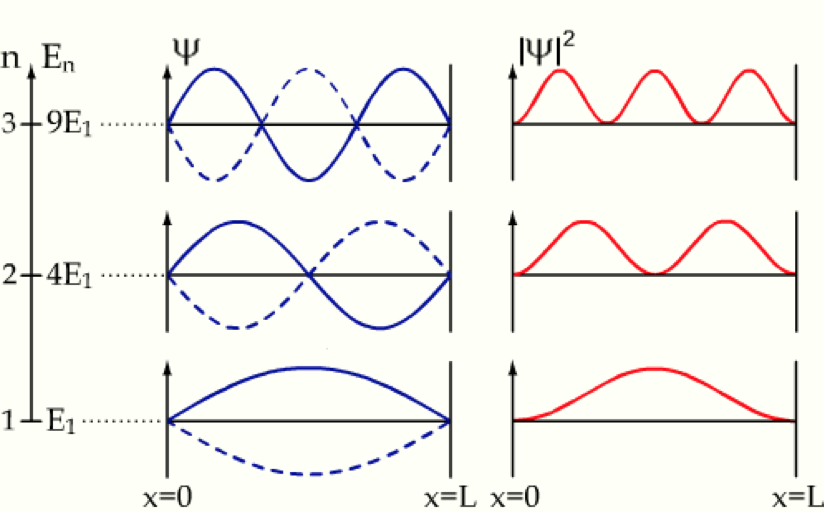
\includegraphics[width=5cm]{./img/potentialtopf.png}  \\ 
\end{center}
	\cookbox{Schrödingergleichung (im eindimensionalen Potentialtopf)}{
		\item Seperation: Ist das Potential zeitunabhängig? Wenn ja $\Ra v(\vec r, t) \ra v(\vec r)$
		\item Bereichseinteilung: 
			\subitem  $x < a$
			\subitem $a < x < b$ (im Topf)
			\subitem $b < x$
		\item Aufstellen der zeitunabhängigen Schrödingergleichung
		\item Ansatz: $\Phi(x) = A e^{\j kx} + B e^{-\j kx}$ oder $A \sin(kx) + B\cos(kx)$
		\item Bestimme Koeffizienten $A, B$ und $k$ über die Randbedingungen
		\item Amplitude aus der Normierungsbedingung bestimmen
		\item Einsetzen und Umformen
		$E = \frac{k^2 \pi^2}{2 m a^2} n^2$ mit $k = \frac \pi a n$
		}
		
\subsubsection*{$\delta$-Dim., unendl., zeitinvar. Potentialtopf: $i=\eset{x,y,...,\delta}$}
	
Lösung der DGL:
$\Psi(\vec r) = \sqrt{\frac{2^\delta}{ \prod L_i }} \prod\limits_{i=1}^\delta \sin(k_i \cdot r_i)$

Energie:  $E_n = \frac{\hbar^2}{2m} \cdot \sum k_i^2$
\subsubsection*{für $\delta = 1$ (eindimensionaler PT)}
\boxed{ E_n = \frac{\hbar^2}{2m} k_n^2 = \frac{h^2 n^2}{8 m L^2} = E_1 n^2 } \quad \boxed{k_n = \frac{n \pi}{L} }
}
% Endlicher Potentialtopf: $k^2 = \frac{2m(E - V)}{\hbar^2}$




\sectionbox{
	\subsection{Moleküle - Bindungstypen}
\tablebox{
	\begin{tabular*}{\columnwidth}{@{\extracolsep\fill}lll@{}}
	\ctrule
			Bindung & Eigenschaften & Energie \\\cmrule
	Ionisch & Elektronaustausch, stark, starr & $\SI{3.4}{\electronvolt}$ \\
	Kovalent & Gemeinsame Elektronen & \\
	Metallisch & "`Elektronensee"' &  \\
	Dipol & Coulombkräfte von Partialladungen  & \\
	\ctrule
	\end{tabular*}
}

\subsubsection{Ionische Bindung }
	\underline{Voraussetzung}: unterschiedliche Atome,leicht zu ionisieren

\cookbox{Ionisierung}{
		\item Anion und Kation ziehen sich an bis auf einen Abstand der Ionenmittelpunkte \\$r_0=(r_{\text{Cl}^-}+r_{\text{Na}^+})$ (bis sich die Elektronenschalen gerade noch berühren)
    	\item Dabei wird die Energie frei: $E_{\ir el}= \int\limits_\infty^{r_0} \frac{-e^2}{4\pi\epsilon_0r^2 }\diff r= \frac{e^2}{4\pi\epsilon_0r_0}$
    	\item Bindungsenergie beträgt $\frac{\SI{3,4}{\electronvolt}}{\text{Ionenpaar}}$ oder $328\frac{\text{kJ}}{\text{Mol}}$
		\item Coulombanziehung nicht gerichtet $\rightarrow$ positive und negative Ionen lagern so dicht aneinander wie möglich $\rightarrow$ Ionenkristall (nicht verformbar)
		\item Elektronen sind an den Ionen lokalisiert $\rightarrow$ keine freien Elektronen vorhanden $\ra $ Isolator
		\item Differenz der Elektronegativität meist $\Delta E>1.7$
}

\subsubsection{Kovalente Bindung}
	Spinabsättigung der äußeren Elektronenschale durch gemeinsame Elektronen
  
	\begin{itemize}
    	\item Valenz-Elektronen zwischen den Atomen lokalisiert
		\item keine Kugelsymmetrische Ladungsverteilung mehr im Atom
		\item Die Anzahl der Elektronen mit umgepaartem Spin zeigt an wie vielfache kovalente Bindungen eingegangen werden können
		\item treten bei und zwischen Elementen der IV. bis VII. Hauptgruppe auf
		\item gerichtete Bindungen $\rightarrow$ mögliche Kristallstrukturen werden eingeschränkt
		\item Differenz der Elektronegativität meist $\Delta E<1.7$
		\item kovalente gebundene Kristalle sind üblicherweise schlechte Leiter 
	\end{itemize}


\subsubsection{Metallische Bindung}
	Sonderfall der kovalenten Bindung, bei der die Valenz-Elektronen nicht lokalisiert sind.
	\begin{itemize}
    	\item Vorwiegend Elemente mit nur wenigen Außenelektronen
		\item freie Elektronen $\ra $ hohe elektrische Leitfähigkeit, hohe Wärmeleitfähigkeit
		\item Bindung nicht gerichtet $\rightarrow$ hohe Packungsdichte 
		\item Bindungen mit gleich- und ungleichartigen Metallen eingegangen werden
		\item Metallische Bindung ist schwächer als die ionische oder kovalente Bindung
		\item Bindungsstärke hängt von der Zahl der Leitungselektronen ab
	\end{itemize}
	
\subsubsection{Dipolbindung}
	\begin{itemize}
		\item zwischen Molekülen mit permanentem Dipolmoment $\rightarrow$ Moleküle mit positiver und negativer Ladung 
		\item Dipole ordnen sich im Dipolfeld der Nachbaratome so an, dass möglichst geringe Abstand und durch die Coulombkräfte gebunden werden 
    \end{itemize}

\subsubsection{Van-der-Waals-Bindung:} 
        \begin{itemize}
        		\item Atome/Moleküle haben kein permanentes Dipolmoment 
				\item Bindung zwischen Dipolen durch statistische Fluktuationen der Ladungsschwerpunkte.
				\item Sehr schwache Bindung
		\end{itemize}
\subsubsection{Wasserstoffbrückenbindung}
	\underline{Vorraussetzung:} Äußere Schale $>$ vier Elektronen, zwischen 2 Atomen.
		\begin{itemize}
				\item Bindungen über Wasserstoffbrücken der Form A-H-A
				\item Das H-Atom geht eine kovalente Bindung mit Atom der Sorte A ein und gibt sein Elektron ab. Das Proton bleibt fest an Reaktionspartner gebunden und bindet nun zusätzlich das andere negative Atom
				\item Bindungsenergie ist gering $(\SI{0,1}{\electronvolt})$    
 		\end{itemize}
}





\sectionbox{
	\subsection{Das Periodensystem (Siehe Seite 4)}	
\tablebox{
	\begin{tabular*}{\columnwidth}{@{\extracolsep\fill}ll@{}}
	\ctrule
		Hauptquantenzahl &
$n = 1, 2, \ldots (= $ K, L, \ldots - Schale $)$ \\
Nebenquantenzahl &
$l = 0, \ldots, n-1$ (= s,p,d,f - Zuständen)\\
Magnetische Quantenzahl &
$m = -l, -l +1, \ldots, l -1 , l$\\
Spinquantenzahl &
$s = \pm \frac{1}{2}$ \\ 
	\ctrule
	\end{tabular*}
}
	Zu jedem Wert n gehören $n^2$ Zustände durch Variation von $l$ und $m$. Außerdem ist jeweils ein Spin $s = \pm \frac 1 2$ möglich.\\
	\textbf{Entartungsgrad:} Kombination der QZ mit gleicher Energie: $2 n^2$
}


%=======================================================================
\sectionbox{
	\subsection{Atome - Hundsche Regeln}
Legen fest, nach welchem Schema jedes einzelne Orbital eines Atoms mit Elektronen besetzt wird.
\begin{enumerate}
\item Die Schale wird so aufgefüllt, dass $\abs{S} = \abs{\sum s_i} = \max$ %mit $s = \pm \frac{1}{2}$ maximal wird
\item Quantenzahl $\abs{L} = \abs{\sum m_i} = \max$
\item Falls die Schale weniger als halbvoll ist:
	\begin{itemize}
		\item Bahndrehimpuls und Spin antiparallel
		\item Gesamtdrehimpuls $J$: $\abs{J} = \abs{\abs{L} - \abs{S}}$
	\end{itemize}
	Falls die Schale mehr als halbvoll ist:
\begin{itemize}
		\item Bahndrehimpuls und Spin parallel
		\item Gesamtdrehimpuls $J$: $\abs{J} = \abs{\abs{L} + \abs{S}}$
	\end{itemize}
\end{enumerate}
Merke: Volle Schalen liefern keinen Beitrag zu $S$, $L$ und $J$
\paragraph{Pauli-Prinzip:}
Alle Elektronen unterscheiden sich in mindestens einer Quantenzahl
\begin{center}
	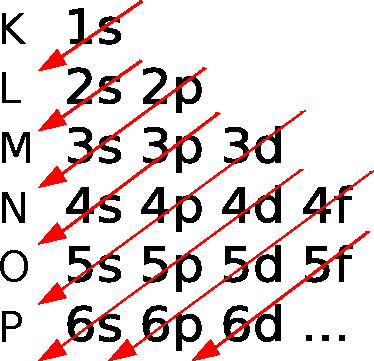
\includegraphics[width = 2cm]{./img/klechkovski.pdf}
\end{center}
{ \fboxsep0.2em
\begin{tabular}{c|ccc}
${}_{\color{red}\displaystyle \boldsymbol{n}}\!{\LARGE \diagdown}\!{}^{\color{blue}\displaystyle \boldsymbol{l}}$ & \color{blue}$0 =\textbf{s}$ & \color{blue}$1 = \textbf{p}$ & \color{blue}$2 = \textbf{d}$\\ \mrule
& $m = 0$ & $m=-1,0,1$ & $m=-2,-1,0,1,2$\\
\color{red}1:K & \fbox{$\uparrow\downarrow$} & \\[0.2em]
\color{red}2:L & \fbox{$\uparrow\downarrow$} & \fbox{$\uparrow\downarrow$}\fbox{$\uparrow\downarrow$}\fbox{$\uparrow\downarrow$}\\[0.2em]
\color{red}3:M & \fbox{$\uparrow\downarrow$} & \fbox{$\uparrow\downarrow$}\fbox{$\uparrow\downarrow$}\fbox{$\uparrow\downarrow$} & \fbox{$\uparrow\downarrow$}\fbox{$\uparrow\downarrow$}\fbox{$\uparrow\downarrow$}\fbox{$\uparrow\downarrow$}\fbox{$\uparrow\downarrow$}\\
\end{tabular} }
} 



\sectionbox{
	\subsection{Kunststoffe}
Bestehen im wesentlichen aus C,H,N und O\\
\textbf{Polymerisation:} Reaktion von Manomeren mit Doppelbindungen zu makromolekularen Ketten\\[0.5em]
\textbf{Polykondensation:} Reaktion von Monomere mit reaktiven Endguppen unter Abspaltung von z.B $H_2O$ oder $HCL$\\[0.5em]
\textbf{Polyaddition:} Venetzung von Epoxiden mit Aminen oder Alkoholen ohne weiteres Reaktionsprodukt\\
}


\sectionbox{
	\subsection{Legierungen und Schmelze}
}

% SECTION ====================================================================================
\section{Mechanische Eigenschaften von Festkörpern}
% ============================================================================================
\symbolbox{
	\begin{tabular*}{\columnwidth}{@{\extracolsep}ll@{}}
		$a_0$ & Gitterkonstante ($ \approx \SI{e-10}{\meter}$) \\
		$N$ & Anzahl Atome in EZ (Anzahl Atome geteilt durch die Zellen,\\
		&   die sich dieses Atom teilen)
	\end{tabular*}


}

\sectionbox{
	\subsection{Dichte}	
Dichte: $\rho = \frac{\diff m}{\diff V} = \frac{m P}{\frac{4}{3} \pi r^3} = \frac{m N}{a_0^3} = \frac{1}{V} 
\frac{N}{N_A} A_r$

$\ra A_r$ in $\si{\kg}$ Umrechnen!

Packungsdichte: $P = \frac{\text{Volumen (Atome)}}{\text{Volumen (Einheitszelle)}} = \frac{N \frac{4}{3} r^3 \pi}{V_{EZ}}$
}

\sectionbox{
	\subsection{Kristallstrukturen}
\begin{tabular*}{\columnwidth}{@{\extracolsep\fill}lll@{}}
	$\underset{\text{simple cubic}}{\text{\large SC/PK}}$ & $\underset{\text{body-centered cubic}}{\text{\large BCC/KRZ}}$ & $\underset{\text{face-centered cubic}}{\text{\large FCC/KFZ}}$\\ \mrule
	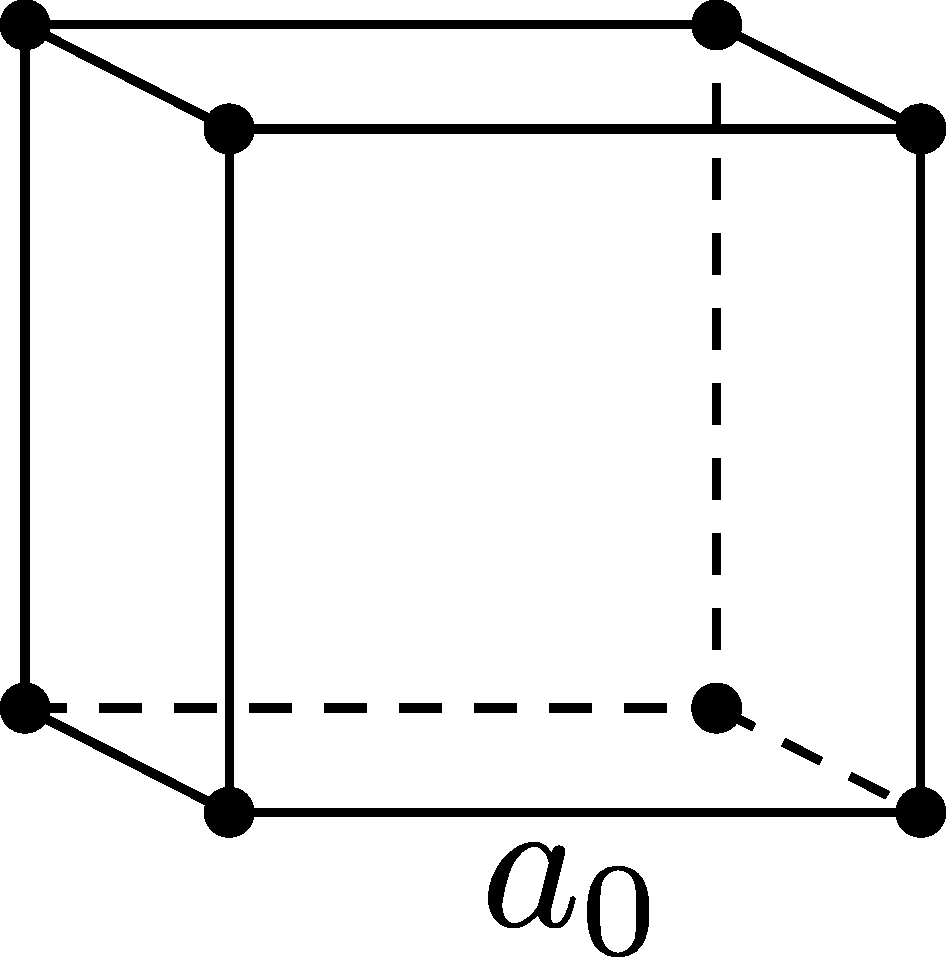
\includegraphics[width = 1.6cm]{./img/sc.pdf} & 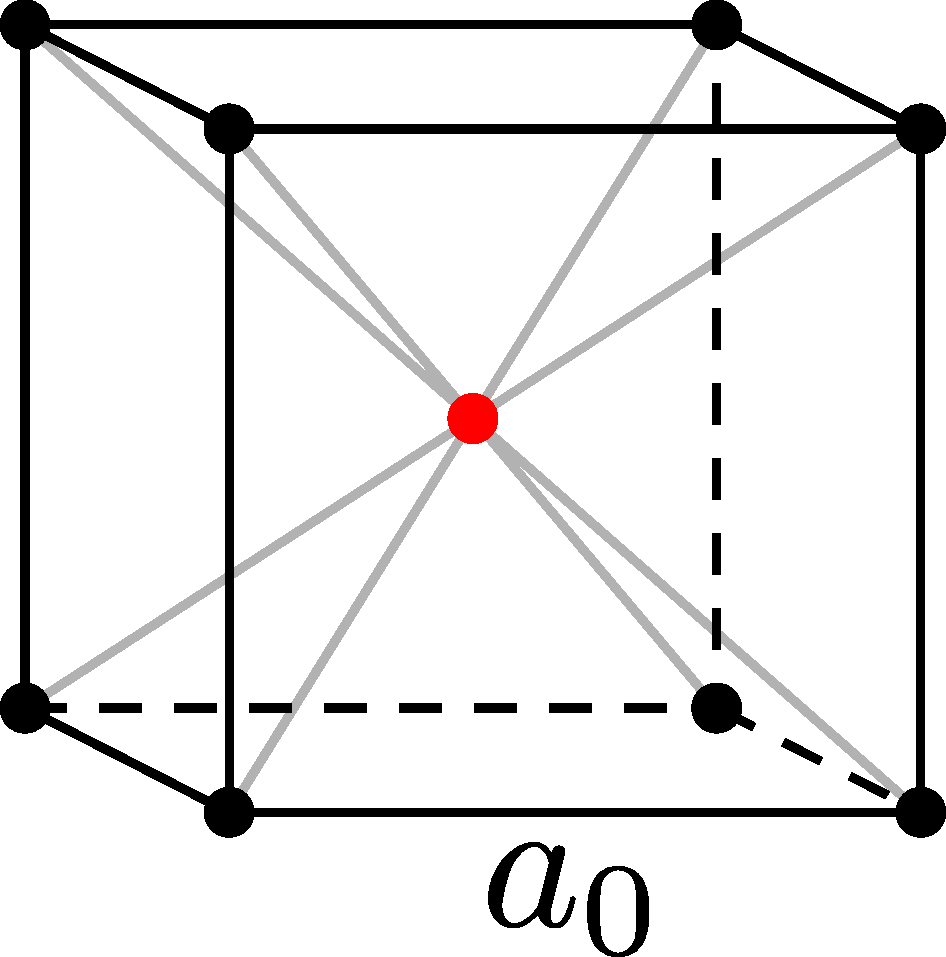
\includegraphics[width = 1.6cm]{./img/bcc.pdf} & 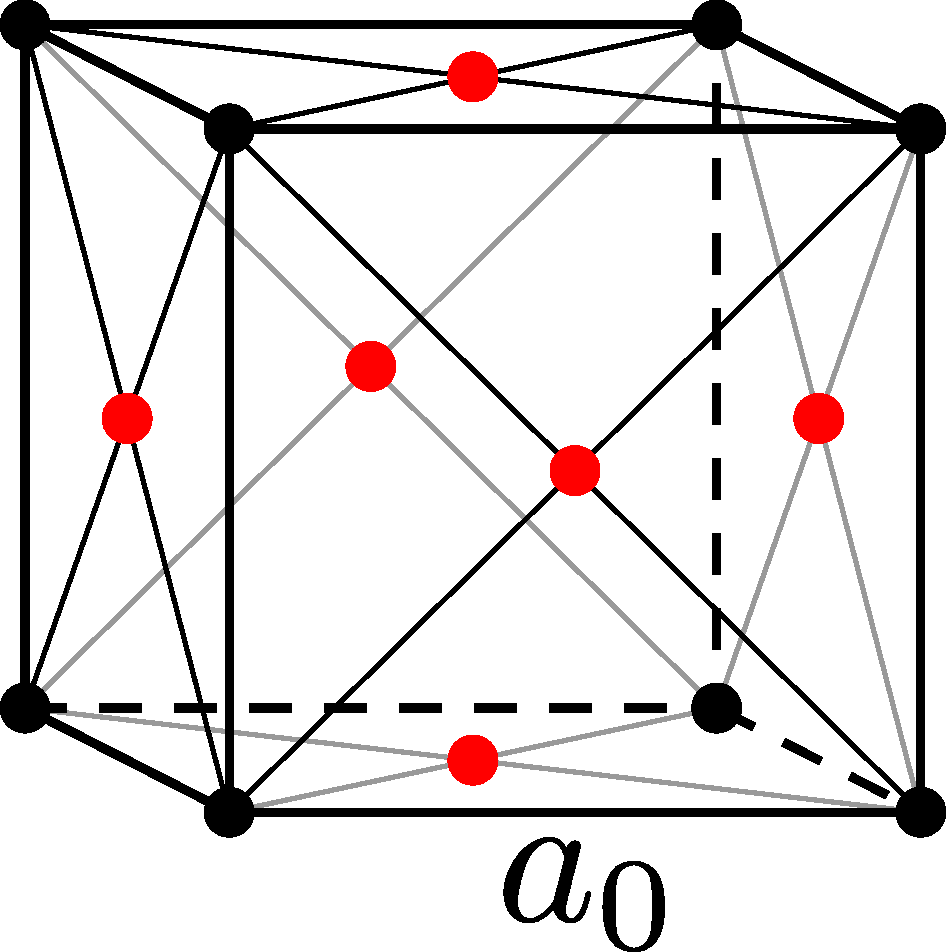
\includegraphics[width = 1.6cm]{./img/fcc.pdf}\\
	$P = \frac{\pi}{6} \approx 0.52$ & $P = \frac{\sqrt{3}\pi}{8} \approx 0.68$ & $P = \frac{\sqrt{2}\pi}{6} \approx 0.74$\\[0.5em]
	$r_{\ir A} = \frac{\sqrt{4}}{4} a_0$ & $r_{\ir A} = \frac{\sqrt{3}}{4} a_0$ & $r_{\ir A} = \frac{\sqrt{2}}{4} a_0$\\[0.5em]
	KZ $=6$ & KZ $=8$ & KZ $=12$\\
	\\
	$\underset{\text{hexagonal}}{\text{\large HCP}}$ & \large Tetraeder & \large Diamant\\ \mrule
	$P = \frac{\pi}{3 \sqrt{2}} \approx 0.74$ & $P = \frac{\pi \sqrt{3}}{16} \approx 0.34$ & $P = \frac{\pi \sqrt{3}}{16} \approx 0.34$\\
	$V_{\ir hex} = \frac{3\sqrt{3}}{2} a^2 h$ & $V_{\ir Tetra} = \frac{\sqrt{2}}{12}a^3$ & $V_{\ir Diamant} = a_0^3$\\
	KZ $=6,12$ & KZ $=4$ & KZ $=4$\\ \\
\end{tabular*}
	 KZ: \textbf{K}oordinations\textbf{z}ahl (Zahl der nächsten Nachbarn)\\
	 Polymorphie: Ein Stoff hat mehrere Kristallgitterstrukturen.
}

\sectionbox{
	\subsection{Elastische Verformung}
\parbox{3.5cm}{ 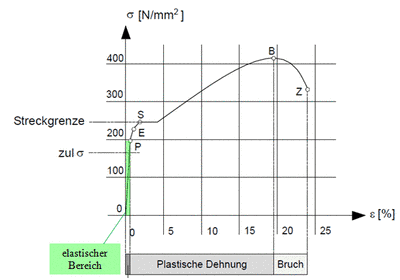
\includegraphics[width=3cm]{./img/spannung-dehnung.png} }
\parbox{3cm}{ Elastizitätsgrenze $\sigma_{\ir E}$ \\ Streckgrenze $\sigma_{\ir S}$ \\ Bruchgrenze $\sigma_B$ ($E = 0$)\\ Bruchdehnung $\varepsilon_B$ \\
	$\ma \varepsilon = \mat{ \varepsilon_{xx} & \varepsilon_{xy} & \varepsilon_{xz} \\ \varepsilon_{yx} & \varepsilon_{yy} & \varepsilon_{yz} \\ \varepsilon_{zx} & \varepsilon_{zy} & \varepsilon_{zz} }$\\
 }

\paragraph{Dehnung}
$\epsilon_{xx} = \frac{\partial u_x}{\partial x}  \quad 
	\epsilon_{yy} = \frac{\partial u_y}{\partial y}	\quad 
	\epsilon_{zz} = \frac{\partial u_z}{\partial z}
$
\paragraph{Scherdeformation}
\[
	\epsilon_{xy} = \frac{\partial u_x}{\partial y} +  \frac{\partial u_y}{\partial x} \quad 
	\epsilon_{yz} = \frac{\partial u_y}{\partial z} + \frac{\partial u_z}{\partial y}\quad 
	\epsilon_{xz} = \frac{\partial u_x}{\partial z}+  \frac{\partial u_z}{\partial x} \quad 
\]

\paragraph{Spannungen}
Normalspannungen $\sigma_{xx}, \sigma_{yy}, \sigma_{zz}$ sind Zug bzw. Druckspannungen. 
Tangentialspannungen (Scherspannungen) $\sigma_{xy}, \sigma_{yz}$


\subsubsection*{Verallgemeinertes Hooksches Gesetz}
\boxed{\ma \sigma = \tensor C \ma \varepsilon} mit $\tensor C$ ist 81 Komponenten Elastizitätstensor 4. Stufe\\
\textbf{Uniaxial:} $\sigma_{xx} = \left( c - \frac{2 \lambda^2}{c + \lambda} \right) \varepsilon_{xx} = E \cdot \varepsilon_{xx}$ \quad $\varepsilon_{xx} = \frac{\Delta l}{l}$\\
$|\vec \sigma| = \frac{|\vec F|}{A} = \frac{EF}{cl} = E \cdot \frac{\Delta l}{l} = \varepsilon E$\\
\\
\textbf{Hydrostatisch:} $(\sigma_{xx} = \sigma_{yy} = \sigma_{zz} = -p)$\\
Kompressionsmodul $K = - V_0 \frac{\diff p}{\diff V} \overset{\text{isotrop}}{=} \frac{E}{3-6\nu}$ \quad Metall $\nu \approx 0.3$\\ 
\\
\textbf{Mikroskopische Ebene:} Bindungskräfte zwischen Atomen\\
Potential $V(r) = - \underbrace{\frac{\alpha}{r^n}}_{\text{anziehend}} + \underbrace{\frac{\beta}{r^m}}_{\text{abstoßend}}$ \qquad $m > n$\\ 
Zw. atomare Kraft $F(r) = - \frac{d V(r)}{dr}$ im GG-Fall $F(r = r_0) = 0$ \\[0.5em]
Elastizitätsmodul $E := - \frac 1 r \frac{dF}{dr} = \sigma \frac{r_0}{\Delta r} = \frac{\sigma}{\varepsilon} = n(m-n) \frac{\alpha}{r_0^{n+3}}$




Akustische Wellen in Festkörpern: $v_{||} = \sqrt{\frac{c}{\rho}}$ \qquad $v_{\perp} = \sqrt{\frac{\mu}{\rho}}$\\
Gitterschwingungen / Phononen: (Für kleine $k$)\\
$\omega_1 = \sqrt{2 c (\frac{1}{M_1} + \frac{1}{M_2})}$ \qquad $\omega_2 = ka\sqrt{ \frac{2 c}{M_1 + M_2}}$
}


% SECTION ====================================================================================
\section{Thermische Eigenschaften von Festkörpern}
% ============================================================================================
	\symbolbox{ 
		\begin{tabular*}{\columnwidth}{@{}lll@{}}
		Druck & $[p]$ & $\si{\newton\per\meter\squared}$ \\
		Seebeck-Ko. & $[S]$ & $\si{\micro\volt\per\kelvin}$\\
		Wärmeleitf. & $[\lambda]$ & $\si{\watt\per\meter\kelvin}$ \\
		Wärmemenge & $[Q]$ & $\si{\joule} = \si{\watt\second}$\\
		Wärmekapazität & $[C]$ & $\si{\joule \per \kelvin}$ \\
		Wärmeleitwert &$[G]$ & $\si{\kelvin \per \watt}$\\
		Innere Energie & $[U]$  & $\si{\joule}$\\
		spez. Wärmekapazität & $[c_{\ir m}]$ & $\si{\joule \per \kelvin \kg}$
	\end{tabular*}
	}
	
\sectionbox{
Wärmekapazität $C = \frac{\partial U}{\partial T} = c n = c_{\ir m} \cdot m = c_{\ir m} \rho V$

Innere Energie $U = 3 N k_{\ir B} T$ \qquad\quad für 1 mol: $\Delta U = \Delta T c_m$

Spezifische Wärme für hohe Temp. $c_m = 3R = \SI{24.9}{\joule\per\mol\kelvin}$

Wärmemenge $Q = CT$

Wärmeleitwert $G = \lambda \frac{A}{l}$

Wärmestrom $\dot Q = -\lambda \grad(T) A = C \dot T = G \Delta T$

Wärmestromdichte $w = \frac{\dot Q}{A} = \frac{\Delta Q}{A \Delta t} = n v c \Delta T = -\lambda \grad(T)$

Phononen: $\lambda_{\ir ph} = \frac{1}{3} C_{\ir ph} v_{\ir Schall} l_{\ir ph}$

Elektronen $\lambda_{\ir el} = \frac{1}{3} C_{\ir el} v_{\ir el} l_{\ir el}$

Mittlere freie Weglänge $l = v \tau$ \qquad\quad $C_{\text{el}} \approx 6n k_B^2 \frac{T}{E_F}$

}

\sectionbox{
		\subsection{Thermische Ausdehnung}
	Ausdehnungskoeffizient $\alpha = \frac{\beta}{3} = \frac{\Delta l}{l} \cdot \frac{1}{\Delta T}$\\
	Volumenänderung: $\frac{\Delta V}{V_0} = 3\alpha \Delta T = \beta \Delta T$\\
	\\
	Grüneisenregel für Metalle: $\alpha \propto \frac{1}{T_S}$ \qquad Schmeltemperatur $T_S$\\
}

\sectionbox{
\subsection{Ideales Gas}
Ideales Gasgesetz: $p V = n_m RT = N k_b T = N_v k_B T$ \\
Kinetische Energie $E_{\ir kin} = \frac{1}{2} m \ol{v^2} = \frac{f}{2} k_{\ir B} T$\\
Teilchendichte: $N = \frac{n \cdot N_{\ir A}}{V} = \frac{\rho N_{\ir A}}{A_r} = \frac{p}{k_{\ir B} T}$ \\ 
Stoffmenge: $n = \frac{N}{N_{\ir A}} = \frac{m}{A_r}$ \qquad Druck $p = \frac{1}{3} N m \ol{v^2}$\\
Gaskonstante: $R = k_b N_{\ir A}= 8,3144 \frac{\text{J}}{\text{mol} \text{ K}}$\\
}

\sectionbox{
		\subsection{Freies Elektronengas}
	Zustandsdichte 3D: \boxed{ D(E) = \frac{1}{V} \frac{\diff Z}{\diff E} = \sqrt[2]{\left( \frac{2m}{\hbar^2} \right)^3} \frac{\sqrt{E}}{2 \pi^2 }}\\
	2D : $D = \frac{m^*}{\pi \hbar^2 a}$ \qquad 1D: $D = \frac{\sqrt{2m^*}}{\pi \hbar a^2} \frac{1}{\sqrt{E - E_{x,j} - E_{z,j}}}$\\
	\parbox{4.3cm}{
	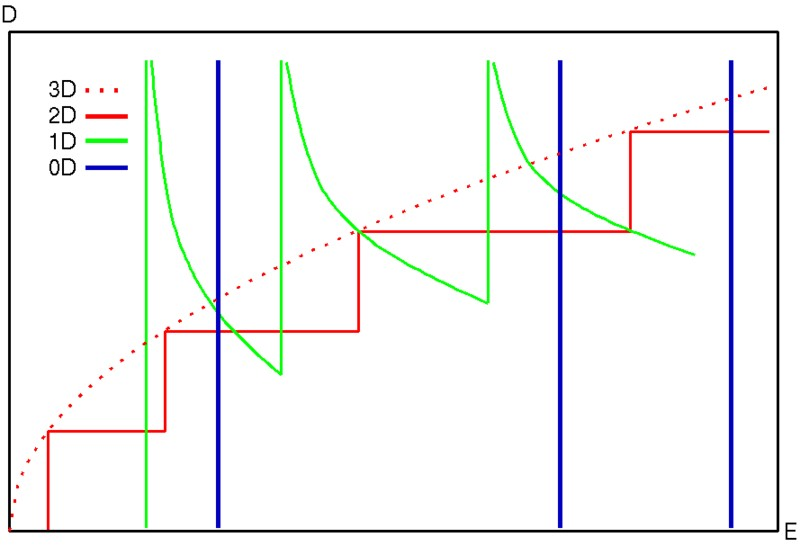
\includegraphics[width = 4.2cm]{./img/dos.jpg} }
	\pbox{5cm}{
	Effektive Masse: \\ \boxed{\frac{1}{m^*} = \frac{1}{\hbar^2} \frac{\diff^2 E(k)}{\diff k^2} }\\ \\ \\
	Wärmeleitfähigkeit: \\ $\lambda_{\ir el} = \frac 1 3 C_{\ir el} v_{\ir el} l_{\ir el}$ }\\
	\\
	Energieeigenwerte: $E_{nml} = \frac{\hbar^2 \vec k^2}{2 m_e^*} = \frac{\hbar^2 \pi^2}{2 m_e^* L^2} (n^2 + m^2 + l^2)$\\
	\\
	Wiedemann-Franzsches Gesetz: \\$\frac{\lambda}{\sigma_{\ir el} T} = L := \frac{\pi^2 k^2_{\ir B}}{3 e^2} = \SI{2.44e-8}{\volt^2\per\kelvin^2}$ \quad ($L:$ Lorentzzahl)
}

\columnbreak

% SECTION ====================================================================================	
\section{Elektrische Eigenschaften von Festkörpern}
%============================================================================================
\symbolbox{ Spez. Wid. $[\rho] = \si{\ohm\meter}$ \quad Leitfäh. $[\sigma] = \si{\per\ohm\meter}$ \quad $[\mu] = \si{\meter\squared\per\volt\second}$ }
\\ \\ 
\sectionbox{
			\subsection{Ladungstransport}
		Je kleiner $a_0$, desto flacher die Potentialbarrieren zwischen den Atomen, desto breiter werden die Energiebänder.
	
		\begin{tabular}{lll}
			& Freies Teilchen & Eingesperrtes Teilchen\\
			$v_{\text{gr}}$ & $\frac{\hbar}{m} k$ & $\frac{1}{\hbar} \frac{\diff E(k)}{\diff k}$\\
			$v_{\text{ph}}$ & $\frac{E}{p}$ &
		\end{tabular}
}
	\sectionbox{
			
		\subsection{Widerstand}
		$R = \rho \frac{l}{A} = \frac{1}{\sigma} \frac{l}{A}$ 
		

		Fermiradius $k_{\ir F} = \frac{\sqrt{2m E_{\ir F}}}{\hbar}$\\
		\boxed{ \sigma = \frac{-en\Delta p_x}{m^* E_x} = n \frac{e^2}{m^*} \cdot \tau }\\

		Elektronen verbinden sich zu Cooper-Paaren

	}		
		\sectionbox{
			\subsection{Elektrochemische Spannung, Korrosion}
		\begin{tabular}{lll}
			kathodisch & $\ra$ edel & $\ra$ positives Potential\\
			anodisch & $\ra$ unedel & $\ra$ negatives Potential\\
		\end{tabular}
		Das unedlere Metall wird zuerst in Wasser mit Efeld aufgelöst
		}\\
			
	
		\sectionbox{
			\subsection{Piezo-Effekt}
		Mechanische Verformung erzeugt elektrische Spannung in Kristallen.\\
		$\vec D = -k_p \frac{F}{AE}$ \quad $\sigma_{xx} = c\frac{\Delta l}{l} + k_p E_x$
		} \\


		\sectionbox{
			\subsection{Pyroelektrizität}
		$\Delta P = \lambda \Delta T$
		}
		


% SECTION ====================================================================================
\section{Thermoelektrische Effekte}
%=============================================================================================
\symbolbox{
	\begin{tabular}{lll}
		elektrische Leitfähigkeit 	& $[\sigma]$ 	& $\si{\siemens \per \meter}$\\
		Wärmeleitfähigkeit			& $[\lambda]$ & $\si{\watt \per \meter \kelvin}$\\
		Seebeck-Koeffizient 		& $[S]$		& $\si{\micro \volt \per \kelvin}$
	\end{tabular} 
}
\sectionbox{
	Durch thermische Teilchenbewegung entsteht eine Diffusionsstromdichte:\\
\boxed{ j_{\ir diff} = -e(n_1 v_{1x} - n_2 v_{2x}) = e \frac{\diff}{\diff T} (D_n \cdot n) \frac{\diff T}{\diff x}}\\
Diffusionskoeffizient $D_n = v_x l_x = v_x^2 \tau$, Fermigeschw. $v_x^2 = \frac{1}{3} v_{\ir F}^2$\\ 
Effektive Teilchengeschw. $\frac{1}{2} m^* v^2 = \frac{1}{2} k_{\ir B} T$\\ 

Seebeck Koeffizient:\\
\boxed{ S := - \frac{e}{\sigma} \frac{\diff}{\diff T} (D_n \cdot n) } \quad \boxed{\Delta U = S \cdot \Delta T}
}
	\sectionbox{
		\subsection{Peltier-Effekt}
	Wärmestromdichte \boxed{ w = \Pi \cdot j} \qquad Peltierkonstante: $\Pi = S \cdot T$\\
	Gütezahl $Z = |\Delta S|^2 \cdot \frac{\sigma}{\lambda}$ mit Gütefaktor $\Delta S = \Pi_1 - \Pi_2$
	}
	
	\sectionbox{
		
	\subsection{Supraleitung}
	Starke Abnahme des Widerstands um Faktor $\le 10^{-14}$ bei einer Sprungtemperatur $T_c$
	
	
	Kritisches Magnetisches Feld: $H_c = H_0 (1 - (\frac{T}{T_C})^2)$ $\ra$ siehe Tabelle Skript S.107
	
	Londongl. $\vec E = \lambda_{\ir L} \dot{\vec j_{\ir s}}$ \qquad $\vec B = -\lambda_{\ir L} \rot \vec j_{\ir s}$
	
	Londonsche Eindringtiefe $\Lambda_{\ir L} = \sqrt{\frac{\lambda_{\ir L}}{\mu_0}}$ \qquad  $\lambda_{\ir L} = \frac{m}{n_{\ir s} e^2}$

	}
		

\columnbreak
% SECTION ====================================================================================	
\section{Halbleiter}
%=============================================================================================
	\symbolbox{
	\begin{tabular}{ll}
		Valenzbandenergie & $E_{\rm V}$\\
		Leitungsbandenergie & $E_{\rm L}$\\
		Bandlückenenergie & $E_{\rm G} = E_{\rm L} - E_{\rm V}$\\
		Fermi-Energie & $E_{\rm F} = k_{\ir B} T_{\ir F} = \frac{\hbar^2}{2m_{\ir e}}(3\pi^2 n)^{2/3}$\\
		Fermi-Temperatur & $T_F = \frac{\hbar^2}{2 m_e k_b} ( 3 \pi^2 n)^{2/3}$
	\end{tabular} }\\
	\\
	\sectionbox{
		Fermi-Verteilung für Elektronen:\\
	\boxed{f_{e}(E,T) = \text{\Large 1} {\boldsymbol{\bigg/}} \left(1 + \exp\left(\frac{E-E_F}{k_B T}\right) \right) }\\
	$f_h(E,T) = 1 - f_e(E,T)$\\
	$E_{\ir F}$: Energieniveau mit Besetzungswahrsch. $0.5$ im thermischen Gleichgewicht.
	Bei $T = \SI{0}{\kelvin}$ entspricht $E_{\ir F}$ dem maximalen Energiezustand eines Elektrons.\\
	$E_{\rm F} = \frac{E_{\rm V} + E_{\rm L}}{2} + \frac{k_{\ir B} T}{2} \ln\left(\frac{N^*_{\ir V}}{N^*_{\ir L}}\right)$\\
	
	
	\boxed{\sigma = n_i e \mu_n + p_i e \mu_p} \qquad $\vec v = \pm \mu \vec E$\\
	mit $n p = n_i^2$ gilt: $0 = n^2 e \mu_n - \sigma n + n_i^2 e \mu_p$ \\ 
	\boxed{m^* \cdot \mu = e \cdot \tau} \qquad \boxed{\frac{1}{\tau} = \frac{1}{\tau_{\ir i}} + \frac{1}{\tau_{\ir ph}} }
	Stromdichte $\vec j = -n e \vec v_{\ir n} + p e \vec v_{\ir p}$
	}
	
	%Zusatzformel: $E_{\ir g}(T) = E_{\ir g}(T = 0) - \frac{\alpha T^2}{T+\beta}$\\
	
	\sectionbox{
		\subsection{Effektive Masse}
	$m^* = \frac{\hbar^2}{\frac{\diff^2 E(k)}{\diff k^2}}$ \qquad $m^* = \sqrt[3]{m_{||}^* m_\perp^{*2}}$ \\
	$m_{\ir h}^* = \left(m^{*\frac{3}{2}}_{\ir hl} + m^{*\frac{3}{2}}_{\ir hh}\right)^{\frac{2}{3}}$	
	%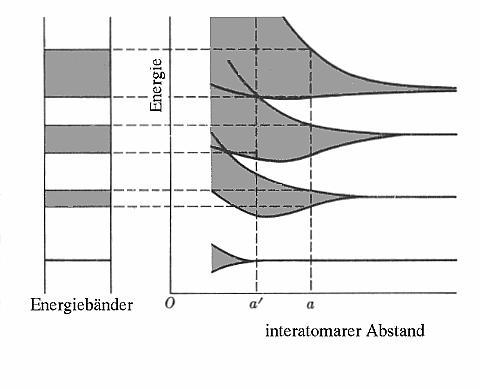
\includegraphics[width = 3cm]{./img/bandstruktur.jpg}\\
	%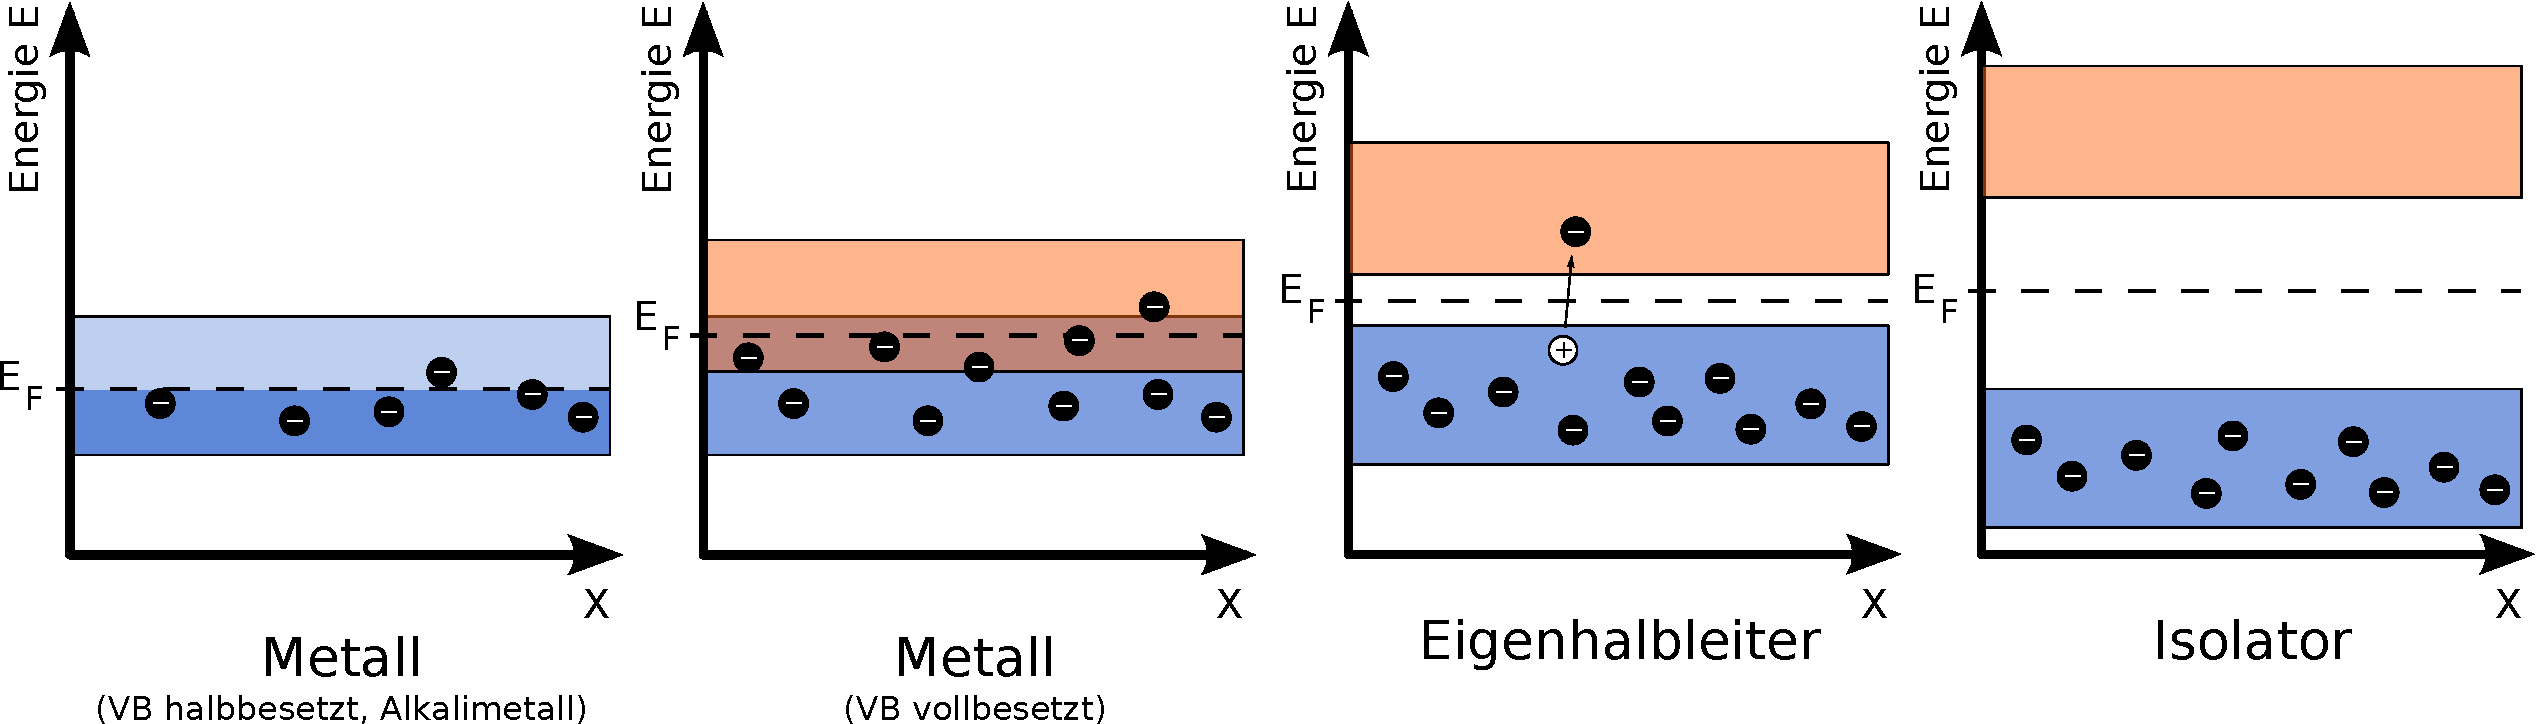
\includegraphics[width = \columnwidth]{./img/energyband.pdf}\\
	%$E_{F,\text{intr}} \approx \frac{1}{2} E_{\ir G}$ \qquad (Metall: $E_{\ir F}$ liegt im Band!)\\
	}
	
	\symbolbox{
	\begin{tabular*}{\columnwidth}{@{}lll@{}}
		Fermi-Verteilung &$f_e$ & $ [\si{1}]$\\
		Elektronen/Löcherdichte& $n,p$ & $ [\si{\per\centi\meter\tothe{3}}]$\\
		Zustandsdichte & $D_{\ir L/V}$ & $ [\si{\per\centi\meter\cubed\electronvolt}]$\\
		effkt. Zustandsdichte Leitungsband & $N_L^*$  & $ [\si{\per\meter\cubed}]$\\
		effkt. Zustandsdichte Valenzband & $N_V^*$ & $ [\si{\per\meter\cubed}]$
	\end{tabular*}
	\begin{tabular*}{\columnwidth}{@{}ll@{}}
			Intrinsische Ladungsträgerdichte & $n_i = \sqrt{N_L^* N_V^*} e^{- \frac{E_g}{2 k_b T}}$ \\ 
	\end{tabular*}

	}
	
\sectionbox{
		\tablebox{
	\begin{tabular*}{\columnwidth}{@{\extracolsep\fill}ll@{}}
	\ctrule
	\textbf{Leitungsband} & \textbf{Valenzband}\\ \cmrule
	Elektronendichte & Löcherdichte\\
	$n = \int\limits_{E_{\ir L}}^\infty D_{\ir L} \cdot f_e \diff E$ & $p = \int\limits_{-\infty}^{E_{\ir V}} D_{\ir V} \cdot f_h \diff E$\\[2em]
	Zustandsdichte  & Zustandsdichte\\
	$D_{\ir L} = \frac{(2 m_n^*)^{3/2}}{2 \pi^2 \hbar^3} \sqrt{E-E_{\ir L}}$ & $D_{\ir V} = \frac{(2 m_p^*)^{3/2}}{2 \pi^2 \hbar^3} \sqrt{E_{\ir V} - E}$\\[2em]
	Effektive Zustandsdichte & Effektive Zustandsdichte\\	
	$N^*_{\ir L} = 2 \left( \frac{m_n^* k_{\ir B} T}{2 \pi \hbar^2}\right)^{3/2}$ & $N^*_{\ir V} = 2 \left( \frac{m_p^* k_{\ir B} T}{2 \pi \hbar^2}\right)^{3/2}$\\
	$n = N^*_{\ir L} \exp\left(-\frac{E_{\ir L} - E_{\ir F}}{k_{\ir B}\cdot T}\right)$ & $p = N^*_{\ir V} \exp\left(-\frac{E_{\ir F} - E_{\ir V}}{k_{\ir B}\cdot T}\right)$ \\ 
	\cbrule
	\end{tabular*}
	}
}


	\emphbox{
	Boltzmann-Näherung: \hfill $f_e(E,T) \approx \exp\left(-\frac{E-E_F}{k_B T}\right)$\\[0.5em]
	Damit gilt: \hfill $n \cdot p = n^2_{\ir i} = N^*_{\ir L} \cdot N^*_{\ir V} \cdot e^{-\frac{E_{\ir g}}{k_{\ir B} T}} $\\[0.5em]
	Dotierungs-Bilanzgleichung: \hfill $n + N_{\ir A}^{-} = p + N_{\ir D}^{+}$\\[0.5em]
	Leitfähigkeit: \hfill $\sigma = n \cdot e \cdot \mu_n + p \cdot e \cdot \mu_p $\\
	}

	\sectionbox{
	\subsection{Dotierung von Halbleitern}		
	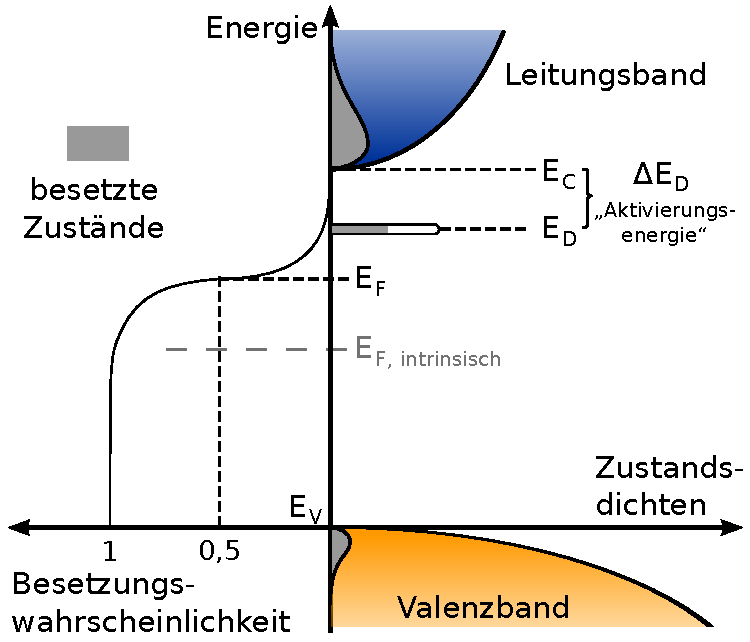
\includegraphics[width = 5cm]{./img/ndotiert.pdf}
	\tablebox{
	\begin{tabular*}{\columnwidth}{l@{\extracolsep\fill}l} \ctrule
	n-Dotierung $+1e^-$ & p-Dotierung $+1h^+$\\ \cmrule
	Donator aus \rom{V} & Akzeptor aus \rom{III}\\
	$N_{\ir D} = N_{\ir D}^0 + N_{\ir D}^+$ & $N_{\ir A} = N_{\ir A}^0 + N_{\ir A}^+$\\
	$N_{\ir A} = 0$ & $N_{\ir D} = 0$\\[1em]
	%$n \approx N_{\ir D}^+$ & $p \approx N_{\ir A}^-$\\ siehe Tempnäherung
	$N_{\ir D}^{0} = N_{\ir D} \cdot f(E_{\ir D},T)$ & $N_{\ir A}^0 = N_{\ir A} [1 - f(E_{\ir A},T)]$\\ 	
	$N_{\ir D}^+ = N_{\ir D} [ 1- f(E_{\ir D},T)]$ & $N_{\ir A}^{-} = N_{\ir A} \cdot f(E_{\ir A},T)$\\ \cbrule
	\end{tabular*} }\\
	Amphoter: Sowohl n- als auch p-Dotierung. Bei \rom{III}-\rom{V} HL: \rom{IV}
	}



	

	\sectionbox{
		\subsection{Temperaturnäherungen für dotierte HL}
	\begin{description}
		\item[niedrige T:] $n \approx \exp(-\frac{E_{\ir L} - E_{\ir D}}{2 k_{\ir B} T})$
		\item[mittlere T:] $n \approx N_D = \const$
		\item[hohe T:] $n \approx n_i$
	\end{description}
	Trick: $\sqrt{N_L^* N_V^*} \sim T^{\frac 3 2}$
	}	

	\sectionbox{
		\subsection{Ausgleichsvorgänge}
		Generationsrate: $G = \underset{\text{Thermisch}}{G_{\ir T}} + \underset{\text{Optisch}}{G_{\ir L}}$\\
		Rekombinationsrate: $R = r(T) n p$
	}
	\sectionbox{
		\subsection{Diffusionsströme}
		$j_{n\!/\!p}^{\ir diff} = e D_{n\!/\!p} \frac{\diff {n\!/\!p}}{\diff x}$ \qquad Einstein Beziehung: $D_{n\!/\!p} = \frac{k_{\ir B} T}{e} \mu_{n\!/\!p}$\\
		Diffusionslänge $L_{n\!/\!p} = \sqrt{D_{n\!/\!p} \tau_{n\!/\!p}}$ \qquad Debye-Länge $L_{\ir D} = \sqrt{D \tau_{\ir R}}$
	}	
	

	
% SECTION ====================================================================================	
\section{Dielektrische Eigenschaften}
% ============================================================================================


	\sectionbox{
	Dielektr. Verschiebung $\vec D = \varepsilon_r\varepsilon_0 \vec E = \varepsilon_0 \vec E (1+\chi^{\ir el}) = \varepsilon_0 \vec E + \vec P$\\
	Komplexe Permittivität: $\varepsilon_r = \varepsilon'_r + \i \varepsilon''_r = \abs{\varepsilon_r} e^{\i \delta}$ \\
	$\varepsilon'(\omega) = \varepsilon_\infty + \frac{\varepsilon_{\ir stat} - \varepsilon_\infty}{1 + \omega^2 \tau^2}$ \qquad $\varepsilon''(\omega) = \frac{\varepsilon_{\ir stat} - \varepsilon_\infty}{1 + \omega^2 \tau^2} \omega \tau$\\
	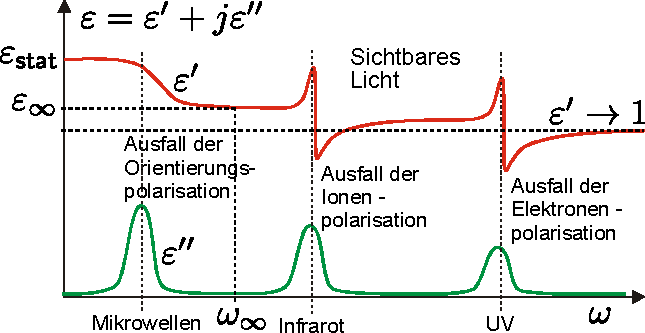
\includegraphics[width = 6cm]{./img/reldie.pdf}
	}
\symbolbox{
	\begin{tabular*}{\columnwidth}{@{}lll@{}}
		Polarisation $[P] = \si{\ampere\second\per\meter\squared}$ & Polarisierbarkeit $[\alpha] = \si{\meter^3}$\\
		Äußeres Feld $\vec E_{\ir ext}$ & Induziertes Gegenfeld $\vec E_{\ir in}$\\
	\end{tabular*}
	}	
\sectionbox{
	\subsection{Polarisation (S. 144)}

	Dipolmoment \boxed{\vec p = \vec s \cdot q = \varepsilon_0 \alpha \vec E_{\ir ext}} \qquad Polarisation \boxed{ \vec P = N \vec p }
	
	Im Kristallgitter $ N = \frac{1}{8 R^3}$
	
	Claudius-Mosotti-Gleichung: $\frac{\alpha N_v}{3} = \frac{\varepsilon_r -1}{\varepsilon_r +1} \Ra  \epsilon_r = 1 + \frac{\alpha N}{1 - \frac{\alpha N }{3}}$
	
	Suszeptibilität $\chi^{\ir el} = \varepsilon_r - 1 = \frac{\vec P}{\varepsilon_0 \vec E} = \frac{\vec P_{in}}{\varepsilon_0 \vec E{\ir in}} = \frac{\alpha N}{1- \frac{\alpha N}{3}}$

	\subsubsection*{Elektronische Polarisation} Elektronenhülle verschiebt sich durch äußeres Feld\\
	$\vec p = \varepsilon_0 \alpha \vec E{\ir ext}$ \qquad Polarisierbarkeit $\alpha = 4\pi R^3$
	
	\subsubsection*{Ionische Polarisation} Ionen werden durch äußeres Feld verschoben\\
	$p = q \Delta r_{\ir Atom} = \varepsilon_0 \alpha E$ \qquad $\alpha = \frac{q^2}{2c \varepsilon_0}$
	
	\subsubsection*{Orientirungspolarisation} Permanente Dipole werden durch E-Feld ausgerichtet.
	$\nu = \frac{E p}{k_B T}$
	Energie eines Dipols: $U(\theta) = -\vec p \vec E = -pE \cdot \cos(\theta)$
	 
	Energieverteilung $w(\theta) = \exp(-\frac{U(\theta)}{k_B T}$
	
	$\ol{\cos(\theta)} = \frac{\ol{w(\theta) \cos(\theta)}}{\ol{w(\theta)}}$
	
}


% SECTION ====================================================================================	
\section{Magnetische Eigenschaften}
% ============================================================================================
	\symbolbox{
	\begin{tabular*}{\columnwidth}{@{}lll@{}}
		Magnetische Flussdichte & $\vec B$ &  $[\si{\tesla}=\si{\volt\second\per\meter\squared}]$ \\
		Magnetische Feldstärke &  $\vec H = \vec M$ & $[\si{\ampere\per\meter}]$\\
		Bahndrehimpuls  & $\vec L$ & $[\si{\volt\ampere\second\squared}]$ \\
		Magnetisches Moment & $\vec m$ & $[ \si{\ampere\meter\squared}]$\\
		magn. Quantenzahl &$m$ od. $M$ \\ 
		Spinquantenzahl &$S$ \\
		gyromagnetisches Verhältnis & $g$ \\
		Gesamtdrehimpuls &$\vec J$ & $[\si{\tesla}=\si{\volt\second\per\meter\squared}]$ \\
		Magnetische Suszepitbilität & $\chi^m$
	\end{tabular*}
	}
\emphbox{
Bohrsches Magneton: $\mu_{\ir B} = \frac{e \hbar}{2 m_{\ir e}} = \SI{9.274e-24}{\ampere\meter\squared}$	
}
	
\sectionbox{
\tablebox{
	\begin{tabular*}{\columnwidth}{@{}lll@{}}
	\ctrule
& Dielektrika & Magnetika\\
\cmrule
Polarisation & $\vec P = \varepsilon_0 \chi \vec E_{\ir netto}$ & $\vec J = \mu_0 \vec M$\\
Flussdichte &$\vec D = \varepsilon_0 \vec E_{\ir netto} + \vec P$ & $\vec B = \mu_0 \vec H + \vec J$\\	
\cbrule
\end{tabular*}
}

\vspace{10pt}

Gesamtdrehimpuls $J = L + S$

permanentes mag. Dipolmoment $M_z = g (- \mu_B ) J$

Magnetische Suszeptibilität $\chi^m = \mu_r - 1 = \frac{1}{\mu_0} \frac{J}{H} = \frac{M}{H}$

Magnetische Flussdichte $\vec B = \mu_r \mu_0 \vec H = \mu_0 \vec H + \vec J = \mu_0(\vec H + \vec M)$
}

\sectionbox{
		\subsection*{Elementare Dipole:}
		Mechanischer Drehimpuls $\vec L = \vec r \times m_0 \vec v = m_0 r^2 \vec \omega$\\
		Magnetisches Moment $\vec m = I \vec A = -\frac{1}{2} e r^2 \vec \omega = - \frac{e}{2m_0} \vec L$\\
		Gyromagn. Verhältnis:  $g = 1+ \frac{J(J+1) + S(S+1) - L(L+1)}{2J(J+1)}$\\ 
		Spezial: $S=0 \Ra g=1$ (unreal) \qquad $L=0 \Ra g=2$
}
			
	\sectionbox{
		\subsection*{Diamagnetismus ($\mu_{\ir r} < 1$)}
	Wirkung der Lorentzkraft. Immer aktiv, wird aber von Para- und Ferromag. überlagert. Temperatur\textbf{un}abhängig.\\
	$\chi_{\ir dia}^{\ir m} = \frac{\vec M}{\vec H} = - \frac{NZ^* e^2 \ol{r^2} \mu_0}{6m_{\ir e}}$
	}
	
	\sectionbox{
		\subsection*{Paramagnetismus ($\mu_{\ir r} > 1$)}
	Material besitzt magnetische Dipolmomente. (Unvollständige Elektronenschalen) 
	
	dominiert oberhalb der Curie-Temperatur
	
	Curiesches Gesetz: $\chi_{\ir para}^{\ir m} = \frac{N \mu_0 g^2 J(J+1)\mu_{\ir B}^2}{3 k_{\ir B} T}$
	}
	\sectionbox{
			
	\subsection*{Leitungselektronen ($\mu_{\ir r} \gg 1$)}
		\parbox{2.2cm}{ $\chi_{\ir para,le}^{\ir m} = \frac{3}{2} \frac{n\mu_0\mu_{\ir B}^2}{k_{\ir B} T_{\ir F}}$
		
		$\chi_{\ir dia,le}^{\ir m} = - \frac{1}{3} \chi_{\ir para,le}^{\ir m}$} $\Bigg\} \chi_{\ir le}^{\ir m} = \chi_{\ir para,le}^{\ir m} + \chi_{\ir dia,le}^{\ir m} = \frac{n\mu_0\mu_{\ir B}^2}{k_{\ir B} T_{\ir F}}$

	(mit $n = \frac{\text{freie } e}{V{\ir ez}}$)
	}

	\sectionbox{
		\subsection*{Ferromagnetismus} ($\mu_r \gg 1$) gekoppelte, parallele Ausrichtung der Momente. Wirkung nur bis Curie-Temp. \\ $E_A = -\mu_0 \int_{V_{Ww}} \vec H_G \vec H_A \diff V$
	
	Curie-Weiss-Gesetz: $\chi^{\ir m} = \frac{C}{T - \Theta}$ mit $\Theta = \frac{E_{\ir F}}{k_{\ir b}}$
	
	Hystereseverluste $w_v = \oint B \diff H$
	}
	\sectionbox{
		\subsection*{Antimagnetismus} gekoppelte, antiparallele Ausrichtung.
	}
\sectionbox{
		\subsection*{Ferimagnetismus} In eine Richtung stärkere Magnetisierung.
	
$\vec m = I A$ ist antiparallel zu $\vec L$
}

\section{Skizzen und Tabellen}
\sectionbox{
\subsection{Skizzen}
\tablebox{
	\begin{tabular*}{\columnwidth}{@{\extracolsep}ll@{}}
	\ctrule
	Name & Seite \\
	\cmrule 
		molare spezifische Wärme &  70	\\
		Thermoelement & 104 \\
		Peltier-Effekt & 105 \\
		Peltier-Element & 105 \\
		Leitfähigkeit/Supraleitung & 106 \\
		Wärmeleitfähigkeit & 75 \\
		Temp. dot. Halbleiter & 122\\
	Berthe-Slater-Kurve &  164 \\
	Magnetische Sättigung & 167\\
	Magnetisierungskurve & 171\\
	Legierungssystem ohne Mischlücke & 42 \\
	Legierungssystem ohne Mischkristallbildung & 44 \\
	Legierungssystem mit Mischlücke & 45 \\
	Legierungssystem mit intermetallischen Verbindungen & 46 \\
	Abstandsabhängigkeit interatomarer Kräfte & 59 \\ 
	Spannungs/Dehnungsdiagramm & 63 \\
	Festigkeit bei wechselnder Belastung & 67 \\ 
	Dotierkonzentrationen & 126 \\
	Hystereskurve eines Ferroelektikums & 149\\
	\cbrule
	\end{tabular*}
}	
}

\sectionbox{
	\subsection{Tabellen / Werte}
	\tablebox{
	\begin{tabular*}{\columnwidth}{@{\extracolsep}ll@{}}
	\ctrule
	Name & Seite \\
	\cmrule 
	Wärmeleitfähigkeit & 75 \\ 
	Thermopaare & 104 \\
	Kritische Feldstärke Supraleiter & 107 \\
	Orbitalebestetzung & 23 \\
	Elektronenhülle & 24 \\
	
	\cbrule
	\end{tabular*}
}	
}


% #### Prüfungsgerüchte ###	

%Warum Benzolringe so wichtig sind
% Ende der Spalten
\end{multicols*}

%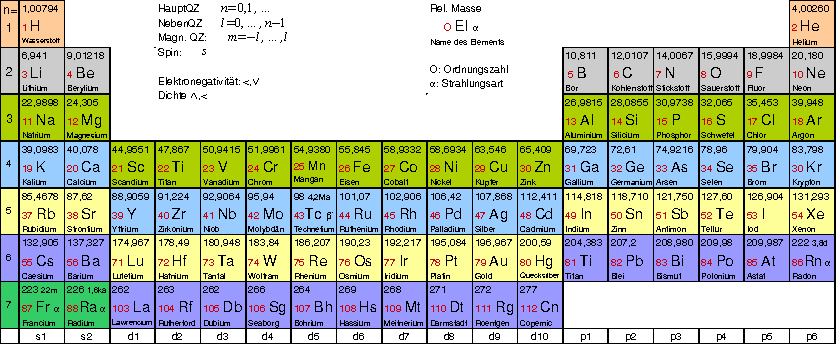
\includegraphics{./img/period.pdf}
\hspace{-5mm}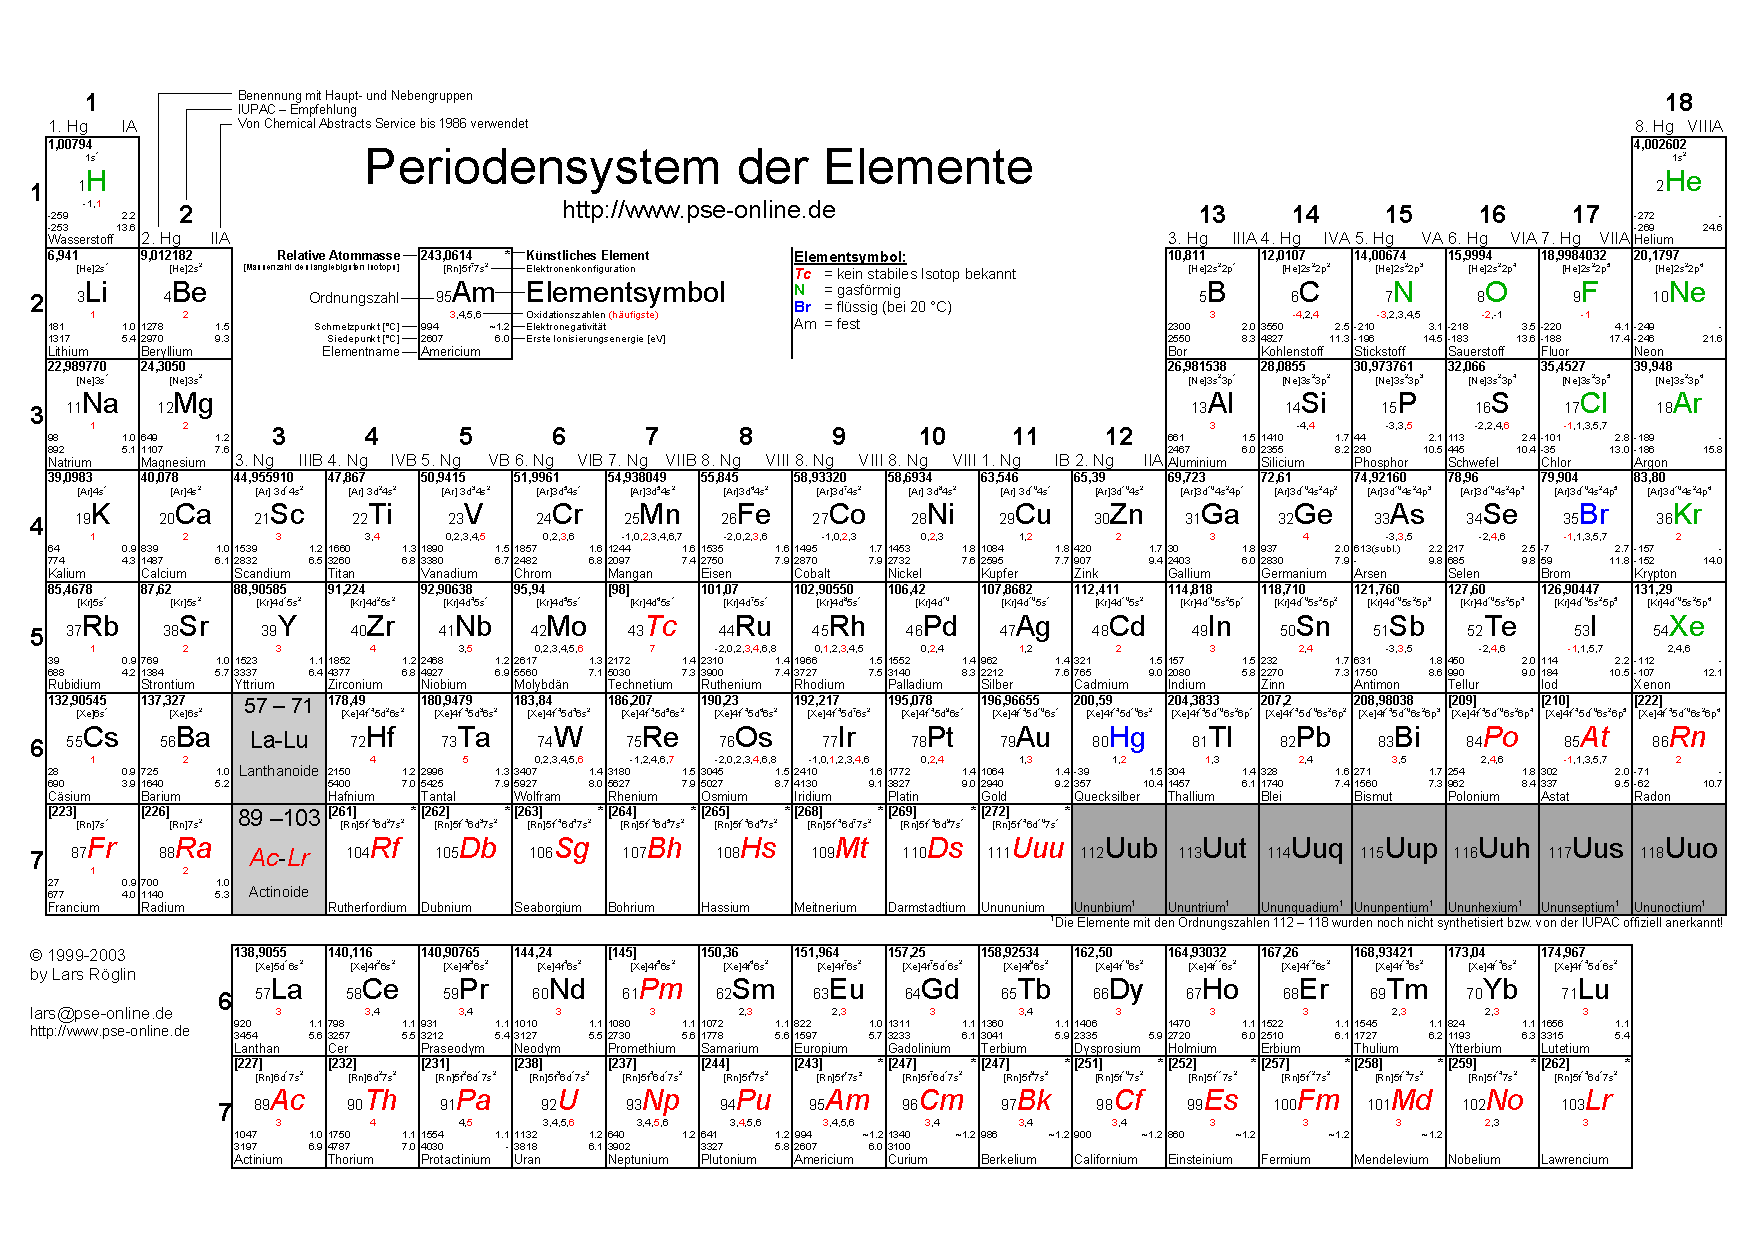
\includegraphics[width = 29.3cm]{./img/pse.pdf}


% Dokumentende
% ======================================================================
\end{document}

% ToDos:
% De-Broglie-Wellenlänge
% Diffusion; Ficksches Gesetz
% Phasendiagramme
% Gibbssche Phasenregel
% Kohlenwasserstoffe
% Mechanische Eigenschaften
% Im Periodensystem markieren welche Elemente welche Magnetismus haben
